\documentclass[12pt,letterpaper]{article}
\usepackage{amsmath,amsthm,amsfonts,amssymb,amscd}
\usepackage{fullpage}
\usepackage{graphicx}
\usepackage{lastpage}
\usepackage{listings}
\lstset{
	numbers=left,
	numbersep=5pt,
	stepnumber=1,
	tabsize=2,
	showstringspaces=false
}
\usepackage{enumerate}
\usepackage{fancyhdr}
\usepackage{hyperref}
\usepackage{mathrsfs}
\usepackage{cancel}
\usepackage{xcolor}
\usepackage[margin=3cm]{geometry}
\setlength{\parindent}{0.0in}
\setlength{\parskip}{0.05in}

% Edit these as appropriate
\newcommand\course{STA561/CS571}
\newcommand\semester{Fall 2013}     % <-- current semester
\newcommand\hwnum{5}                  % <-- homework number
\newcommand\yourname{Matt Dickenson} % <-- your name
\newcommand\login{mcd31}           % <-- your NetID
\newcommand\hwdate{Due: 28 October, 2013}           % <-- HW due date

\newenvironment{answer}[1]{
  \subsubsection*{Problem #1}
}


\pagestyle{fancyplain}
\headheight 35pt
\lhead{\yourname\ \texttt{\login}\\\course\ --- \semester}
\chead{\textbf{\Large Homework \hwnum}}
\rhead{\hwdate}
\headsep 10pt

\begin{document}

\noindent \emph{Homework Notes:} I did not work with anyone else on this homework or refer to resources other than the course notes, textbook, and course Piazza page.

\begin{answer}{1}

\paragraph{A} Figure \ref{eigens} shows the distribution of eigenvalues for each matrix covariance matrix of $X$ with different values of $\psi$ ($X_i$ uses $\psi_i$). All of the distributions are right-skewed, but the mean of the eigenvalues increases and the variance decreases as the amount of noise ($\psi$) in the original matrix increases. The eigenvalues were normalized using the $\ell^2$ norm. 

\begin{figure}[h!]
\begin{center}
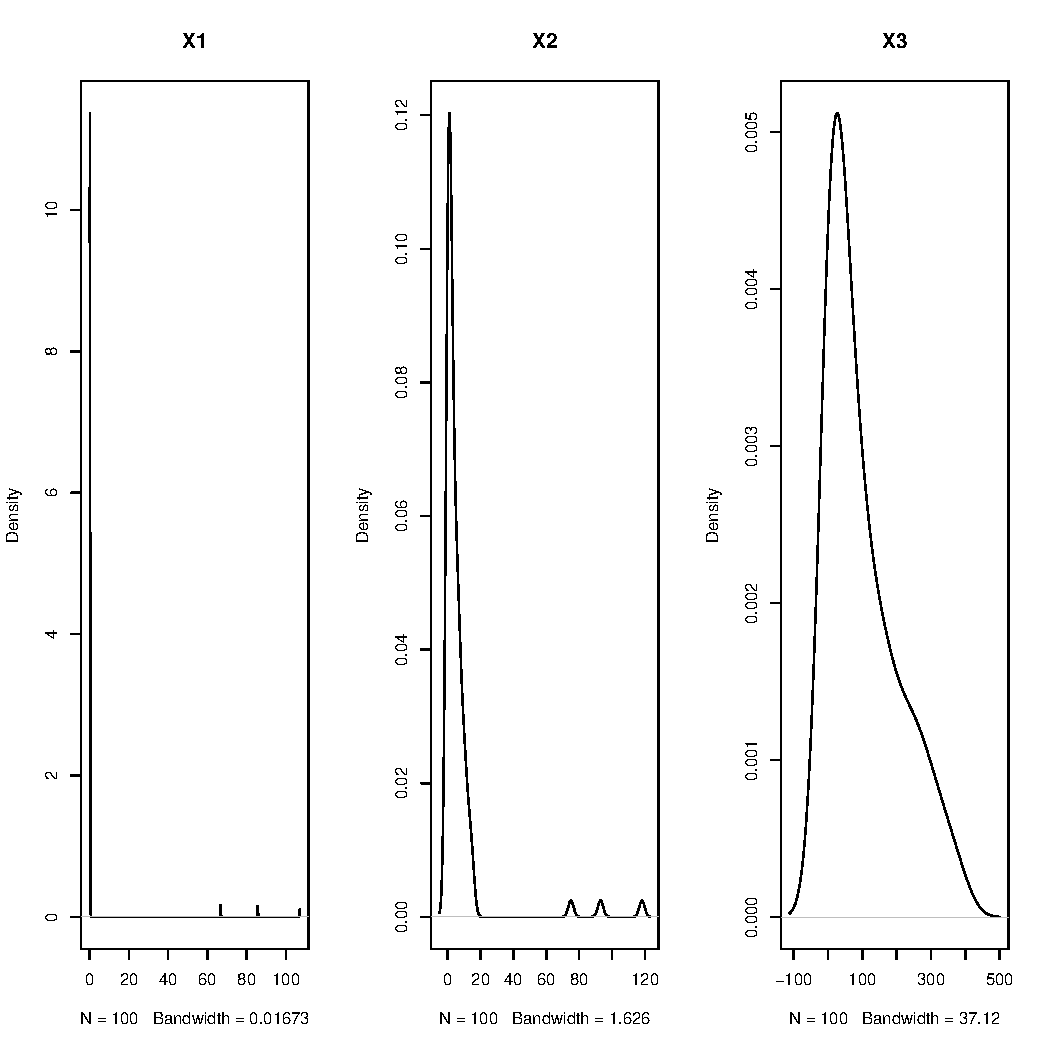
\includegraphics[scale=0.5]{1a.pdf}
\caption{Distribution of Normalized Eigenvalues for Three Values of $\psi$}
\label{eigens}
\end{center}
\end{figure}

\paragraph{B} Table \ref{rmse} presents the root mean squared error (RMSE) between the covariances of the X matrices and the matrix reconstructions using the first three eigenvectors (and eigen values). Overall, the eigenvectors do a good job of recapitulating the original data matrices. Those with less noise (small $\psi$) do a better job (lower RMSE) than those with more noise. 

\begin{table}[h!]
\begin{center}
\caption{RMSE between Cov(X) and Matrix Reconstructions}
\label{rmse}
\begin{tabular}{cr}
$\psi$ & \texttt{RMSE} \\
\hline
0.2 & 0.0054 \\
2 & 0.553 \\
10 & 13.029
\end{tabular}
\end{center}
\end{table}

\paragraph{C} When we reconstruct the matrices we are able to obtain an estimate of the covariance of $X$, subject to some noise. This could be useful for identifying the number of components that could be used in our analysis, as long as we assume that the level of noise is relatively low. 

\end{answer}


\end{document}